\documentclass[conference,letterpaper,10pt]{IEEEtran}
\IEEEoverridecommandlockouts

\usepackage{cite}
\usepackage{amsmath,amssymb,amsfonts}
\usepackage{graphicx}
\usepackage{booktabs}
\usepackage{array}
\usepackage{textcomp}
\usepackage{xcolor}
\usepackage{tikz}
\usetikzlibrary{positioning,arrows.meta,fit,backgrounds}
\usepackage{url}
\usepackage[hidelinks]{hyperref}
\usepackage{stfloats}
\usepackage{adjustbox}
\usepackage[section]{placeins} % keeps every figure/table inside its own section
\graphicspath{{figures/}}

% Let tables and figures sit close to the text that discusses them.
\renewcommand{\topfraction}{0.9}
\renewcommand{\bottomfraction}{0.8}
\renewcommand{\textfraction}{0.07}
\renewcommand{\floatpagefraction}{0.85}
\renewcommand{\dbltopfraction}{0.9}
\renewcommand{\dblfloatpagefraction}{0.85}
\setcounter{topnumber}{3}
\setcounter{bottomnumber}{2}
\setcounter{totalnumber}{5}
\setcounter{dbltopnumber}{2}

\begin{document}

\title{An Energy-Aware Evaluation Framework for Selecting Sustainable Machine Learning Models in Cloud Data Centers}

\author{
\IEEEauthorblockN{Md. Israfil Hossain (0112230585)$^{*}$, Ashiq Anzum (0112230567)$^{*}$, Navia Ferdous Nowrin (0112230990)$^{*}$,\\
Naimur Rahman Nayeem (0112230569)$^{*}$, Taiamun Erabi Rafin (0112231047)$^{*}$, Nur Amin (0112230943)$^{*}$}
\IEEEauthorblockA{$^{*}$Department of Computer Science and Engineering, United International University, Dhaka, Bangladesh\\
Course: EEE 4261 (E): Green Computing}
}

\maketitle

% =====================================================================
\begin{abstract}
Cloud operators use machine learning (ML) to forecast the CPU load of virtual machines (VMs), which allows them to consolidate workloads and switch off idle servers. These forecasting models are usually chosen on prediction accuracy alone, even though the models themselves consume computing time and energy, and the most accurate model on familiar machines may perform poorly on new ones. We propose an energy-aware evaluation framework that assesses each candidate model on four dimensions: prediction accuracy, computational cost, energy and carbon emissions (measured with CodeCarbon), and robustness across random seeds and unseen VMs. The TOPSIS multi-criteria method then combines these criteria into a single ranking. We apply it to six models, ranging from Linear Regression to tree ensembles and an LSTM network, using real production traces of 50 VMs from the public GWA-T-12 Bitbrains dataset and a further 100 VMs held out for testing. Gradient-boosted trees are the most accurate (LightGBM: mean absolute error 0.664 percentage points, $R^2$ 0.941) and need 22--28 times less training energy than the LSTM and Random Forest, which rank last under every weighting. Fifty-three minutes of hyperparameter tuning improve accuracy by at most 1.5\%. On unseen VMs the ranking reverses, because tree ensembles rely on VM-specific disk and network features; removing these features cuts LightGBM's error on unseen VMs by 30\%. A robustness-aware ranking captures this effect and changes the recommended model. The framework gives cloud providers a transparent, reproducible way to choose forecasting models that are accurate, efficient and robust.
\end{abstract}

\begin{IEEEkeywords}
Green AI, sustainable machine learning, cloud data centers, workload forecasting, energy efficiency, carbon emissions, TOPSIS, multi-criteria decision making, model selection
\end{IEEEkeywords}

% =====================================================================
\section{Introduction}
\label{sec:intro}

Data centers consumed an estimated 1--1.3\% of global electricity in recent years, and growth driven by cloud and AI workloads is projected to raise U.S. data-center demand to 4.6--9.1\% of national electricity by 2030 \cite{masanet2020recalibrating,epri2024powering,ifri2025ai}. A widely used way to reduce this demand is predictive resource management. If an operator knows that a virtual machine (VM) will need little CPU in the next few minutes, the VM can be moved onto a shared physical server and the freed server can be switched off; if a VM is about to become busy, capacity can be reserved in time \cite{panwar2024ml,janardhanan2024load}. Machine learning (ML) has become the standard tool for producing such short-term forecasts \cite{kollu2024comparative,mughees2025stlf}.

The forecasting models themselves, however, also consume computing resources and energy. Research on \emph{Green AI}, which studies the energy cost of AI systems, has shown that the choice of model can change this cost by orders of magnitude, often with little or no gain in accuracy \cite{schwartz2020green,strubell2019energy,luccioni2024power,vente2024clicks}. In the data-center energy literature, by contrast, models are selected almost exclusively on prediction accuracy. In the fifteen recent studies reviewed for this work (Section~\ref{sec:related}), few report training or prediction time, the energy used by the model itself is almost never measured, datasets and metrics differ widely, and none offers a practical procedure for weighing accuracy against cost. A second, less discussed risk is robustness: in practice a forecasting model is applied to many machines, including machines it never saw during training, and the model that is most accurate on its training machines is not necessarily the most accurate on new ones.

\textbf{Gap.} To our knowledge, no prior study chooses workload-forecasting models for data centers with a single decision procedure that weighs prediction accuracy, the computational cost and measured energy of the models themselves, their stability, and their accuracy on unseen machines. Green AI studies measure model energy, but in other domains \cite{vente2024clicks,luccioni2024power}, and multi-criteria model selection has so far relied on error measures alone \cite{koubaa2024mcdm}. This paper brings these concerns together for cloud workload forecasting.

\textbf{Contributions.}
\begin{itemize}
  \item \textbf{A reproducible evaluation framework} that measures each model's accuracy, training and prediction time, energy and CO$_2$ emissions (with CodeCarbon \cite{courty2024codecarbon}), stability across random seeds and accuracy on unseen VMs, and ranks the models with TOPSIS \cite{hwang1981topsis} under several weighting scenarios.
  \item \textbf{A controlled comparison} of six classical, ensemble and deep-learning models on real production traces from the public Bitbrains dataset \cite{shen2015bitbrains}. Gradient-boosted trees reach the best accuracy at a small fraction of the energy of an LSTM or a Random Forest, and extensive hyperparameter tuning buys little.
  \item \textbf{Evidence of a generalization reversal}: the most accurate models on known VMs are among the least accurate on unseen VMs, because they rely on VM-specific disk and network features. Restricting the models to features that do not identify a particular VM largely removes the problem.
  \item \textbf{Practical guidance} for operators, supported by a robustness-aware variant of the ranking, a fleet-scale energy projection and statistical significance tests.
\end{itemize}

Section~\ref{sec:related} reviews related work, Sections~\ref{sec:dataset} and~\ref{sec:method} describe the data and the method, Section~\ref{sec:results} presents and discusses the results, and Sections~\ref{sec:limitations} and~\ref{sec:conclusion} cover limitations, future work and conclusions.

% =====================================================================
\section{Related Work}
\label{sec:related}

\subsection{ML for Data-Center Energy and Workload Forecasting}
Several recent studies forecast data-center power or workload. Mughees \textit{et al.} \cite{mughees2025stlf} forecast the short-term power draw of an AI data center from GPU logs of the MIT Supercloud system, using recurrent (LSTM, GRU) and one-dimensional convolutional networks, and reach an $R^2$ of 0.96. Tariq \cite{tariq2025nextgen} compares Random Forest, XGBoost and an LSTM for cooling optimization on a simulated dataset, and Enyinnah \textit{et al.} \cite{enyinnah2022lstm} report that an enhanced LSTM outperforms the classical ARIMA time-series model and support vector regression on data generated with the EnergyPlus simulator. Afrianto \textit{et al.} \cite{afrianto2025yugo} combine gradient boosting with linear regression to predict server power from hypervisor load. Closest to our setting, Kollu \cite{kollu2024comparative} compares four neural networks (a multilayer perceptron, an autoregressive network, a CNN and an LSTM) for CPU and memory forecasting on the same Bitbrains trace and finds the simple multilayer perceptron most accurate. Beyond forecasting, AI is used for load balancing \cite{janardhanan2024load}, green networking \cite{ebadinezhad2025green}, and multi-agent reinforcement learning that jointly controls cooling, IT load and batteries to cut carbon \cite{sarkar2024carbon}; surveys and reports describe the broader landscape \cite{panwar2024ml,epri2024powering,ifri2025ai,huang2026aidc}. Related forecasting work in adjacent domains covers campus buildings \cite{fathi2020campus} and smart grids \cite{aljarrah2024smartgrid}. All of these studies evaluate models by accuracy; none measures the energy consumed by the forecasting models themselves.

\subsection{Classical Versus Deep Learning}
Deep learning is often assumed to be the best choice for time series, but systematic benchmarks question this. Grinsztajn \textit{et al.} \cite{grinsztajn2022tree} show that tree-based models such as XGBoost remain the most accurate option on medium-sized tabular data, even before their lower cost is taken into account, and Zeng \textit{et al.} \cite{zeng2023transformers} find that simple one-layer linear models outperform far larger Transformer forecasters on nine benchmarks. These results motivate comparing a deep-learning model against simple and ensemble baselines on cost as well as on accuracy.

\subsection{Green AI and the Energy Cost of ML}
Strubell \textit{et al.} \cite{strubell2019energy} and Schwartz \textit{et al.} \cite{schwartz2020green} argued that efficiency should be reported alongside accuracy. Luccioni \textit{et al.} \cite{luccioni2024power} measured order-of-magnitude differences in inference energy across model categories, and Vente \textit{et al.} \cite{vente2024clicks} found that deep-learning recommender systems emit about 42 times more CO$_2$ than traditional ones without consistently better accuracy. Da Silva Barros \textit{et al.} \cite{barros2025small} estimate that selecting appropriately sized models could reduce global AI energy use by about 28\%. Measurement tools such as CodeCarbon \cite{courty2024codecarbon} make such accounting practical; they follow real consumption patterns well, although absolute estimates can deviate by up to 40\% from external meters \cite{bouza2023estimate,fischer2025groundtruth}.

\subsection{Multi-Criteria Model Selection}
Multi-criteria decision making (MCDM) offers a principled way to choose between options that are good on different, conflicting criteria. TOPSIS \cite{hwang1981topsis}, one of the most widely used MCDM methods, ranks the options by how close each one is to an ideal option that would be best on every criterion. Koubaa \textit{et al.} \cite{koubaa2024mcdm} combine TOPSIS with the Analytic Network Process to select electricity-demand forecasting models from several error measures. To our knowledge, MCDM has not been used to select workload-forecasting models on accuracy, computational cost, measured energy and robustness together.

\subsection{Research Gap}
Table~\ref{tab:litgap} compares representative studies against the criteria covered by our framework. Four gaps emerge:
\begin{enumerate}
  \item most studies evaluate prediction accuracy only;
  \item training and prediction cost, and especially the energy and CO$_2$ of the model itself, are rarely measured;
  \item datasets and metrics differ between studies and are often simulated or private, which makes results hard to compare;
  \item no study offers a decision procedure that weighs accuracy, efficiency, sustainability and robustness together, or checks whether the chosen model still works on machines it has not seen.
\end{enumerate}

\begin{table}[!htb]
\centering
\caption{Comparison With Related Work}
\label{tab:litgap}
\footnotesize
\setlength{\tabcolsep}{3pt}
\begin{adjustbox}{max width=\columnwidth}
\begin{tabular}{lcccccc}
\toprule
Work & Real & Acc. & Time & Energy & MCDM & Unseen \\
\midrule
Mughees \textit{et al.} \cite{mughees2025stlf} & \checkmark & \checkmark & -- & -- & -- & -- \\
Tariq \cite{tariq2025nextgen} & sim. & \checkmark & -- & -- & -- & -- \\
Enyinnah \textit{et al.} \cite{enyinnah2022lstm} & sim. & \checkmark & -- & -- & -- & -- \\
Afrianto \textit{et al.} \cite{afrianto2025yugo} & \checkmark & \checkmark & -- & -- & -- & -- \\
Kollu \cite{kollu2024comparative} & \checkmark & \checkmark & -- & -- & -- & -- \\
Sarkar \textit{et al.} \cite{sarkar2024carbon} & sim. & -- & -- & DC$^a$ & -- & -- \\
Koubaa \textit{et al.} \cite{koubaa2024mcdm} & \checkmark & \checkmark & -- & -- & \checkmark & -- \\
Vente \textit{et al.} \cite{vente2024clicks} & \checkmark & \checkmark & -- & \checkmark & -- & -- \\
\midrule
\textbf{This work} & \checkmark & \checkmark & \checkmark & \checkmark & \checkmark & \checkmark \\
\bottomrule
\end{tabular}
\end{adjustbox}
\par\vspace{3pt}
{\scriptsize Real: \checkmark\ = real measured data; sim.\ = simulated data. Acc.: prediction accuracy. Time/Energy: training or inference time and energy/CO$_2$ of the ML model itself. MCDM: multi-criteria model selection. Unseen: test on machines or sites excluded from training. $^a$DC: reduces the carbon of the data center (DC), not of the ML model.\par}
\end{table}

% =====================================================================
\section{Dataset}
\label{sec:dataset}

\subsection{GWA-T-12 Bitbrains Traces}
We use the \emph{fastStorage} trace of the GWA-T-12 Bitbrains dataset \cite{shen2015bitbrains}, published in the Grid Workloads Archive \cite{iosup2008gwa}. Bitbrains is a managed hosting provider for enterprises in the financial sector, including banks, credit-card operators and insurers. The trace contains monitoring data of 1{,}250 VMs connected to fast storage, recorded every 5 minutes between 12~August and 11~September 2013 (about 8{,}600 readings per VM). Each reading has 11 numeric fields: timestamp, number of CPU cores, CPU capacity (MHz), CPU usage (in MHz and as a percentage of capacity), allocated and used memory (KB), disk read and write throughput, and network receive and transmit throughput (KB/s). In other words, every VM provides a multivariate time series of real production resource usage. We verified the format before parsing: every file carries a header row, fields are separated by a semicolon and a tab, and timestamps are in seconds despite the ``[ms]'' header label. Fig.~\ref{fig:split} shows the CPU trace of a typical VM.

\begin{figure}[!htb]
\centering
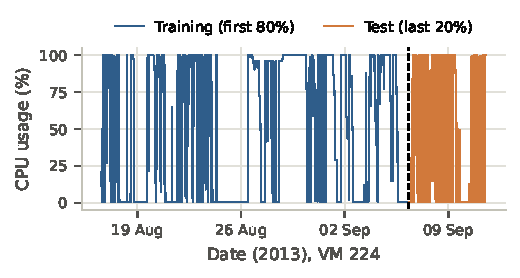
\includegraphics[width=\columnwidth]{fig_split_col.pdf}
\caption{Chronological train/test split for one main-pool VM (VM 224). Every VM is split in the same way, so test data always follow training data in time.}
\label{fig:split}
\end{figure}

\subsection{Data Quality and Cleaning}
The VM IDs were shuffled with a fixed random seed (42), so that the selection can be reproduced, and split into two separate pools: one for the main experiment and one kept aside for the generalization test. We cleaned 150 candidate VMs per pool so that each pool retains at least 100 usable VMs after cleaning. Before cleaning, the 2{,}663{,}335 raw rows contained no missing values but 103{,}458 exact duplicates. 13.8\% of rows reported zero cores and zero memory, i.e.\ the VM was powered off, and 2.7\% reported CPU usage slightly above 100\% (up to 108.5\%), reflecting brief over-commitment. Table~\ref{tab:cleaning} lists the cleaning steps and their effect. Two of them needed a decision:
\begin{itemize}
  \item \textbf{Powered-off periods.} Deleting only the powered-off rows of an otherwise active VM would join readings that are days apart and corrupt the lag features. VMs that were powered off for more than 10\% of the period were therefore excluded (35 VMs) and replaced by the next candidates in the shuffled pool.
  \item \textbf{CPU above 100\%.} These values were capped at 100\% instead of deleted (32{,}131 values), so that the busiest periods, which matter most for provisioning, stay in the series.
\end{itemize}
After cleaning, 99.87\% of consecutive readings are 300$\pm$10\,s apart and the longest gap is 35 minutes.

\begin{table}[!htb]
\centering
\caption{Data Cleaning Steps (300 Candidate VMs)}
\label{tab:cleaning}
\footnotesize
\setlength{\tabcolsep}{4pt}
\begin{adjustbox}{max width=\columnwidth}
\begin{tabular}{cp{3.0cm}rrp{1.55cm}}
\toprule
\# & Rule & Rows removed & VMs & Note \\
\midrule
1 & Remove duplicate rows & 103,458 & 300 &  \\
2 & Remove duplicate (vm\_id, timestamp) & 53 & 300 &  \\
3 & Drop rows missing CPU/memory/timestamp & 0 & 300 &  \\
4 & Fill missing disk/network with 0 & 0 & 300 & 0 cells filled \\
5 & Exclude VMs powered off $>$ 10\% of time & 392,998 & 265 & 35 VMs excluded \\
6 & Remove remaining powered-off rows & 725 & 265 &  \\
7 & Cap CPU\% above 100 at 100 & 0 & 265 & 32,131 values capped \\
8 & Remove other out-of-range values & 78 & 265 &  \\
9 & Exclude VMs with $<$ 100 readings & 7 & 264 & 1 VMs excluded \\
\bottomrule
\end{tabular}
\end{adjustbox}
\end{table}


\subsection{Sampling and Data Split}
The main experiment uses the first 50 VMs of the main pool (401{,}718 readings) and the generalization test uses 100 VMs of the second pool (817{,}478 readings); no VM appears in both. Each main-pool VM is split by time rather than at random: the first 80\% of its readings form the training set (321{,}115 rows in total) and the last 20\%, roughly the final week, form the test set (80{,}303 rows), as illustrated in Fig.~\ref{fig:split}. A time-based split mirrors real use, where a model trained on the past must predict the future. The workloads are bursty and often idle: the median CPU utilization is below 1\%, and 37.4\% of the test values are below 1\%.

% =====================================================================
\section{Methodology}
\label{sec:method}

\subsection{Framework Overview}
Fig.~\ref{fig:pipeline} gives an overview of the framework. The cleaned traces are turned into training examples, six models are trained and tuned, and every model is then evaluated on four dimensions: prediction accuracy, computational efficiency, environmental sustainability and robustness. TOPSIS combines these criteria into one ranking, and a sensitivity analysis checks how much the ranking depends on the weight given to each criterion. Every step is implemented as an independently runnable notebook with its own log, and all reported numbers were produced on the same hardware.

\begin{figure}[!htb]
\centering
\resizebox{\columnwidth}{!}{%
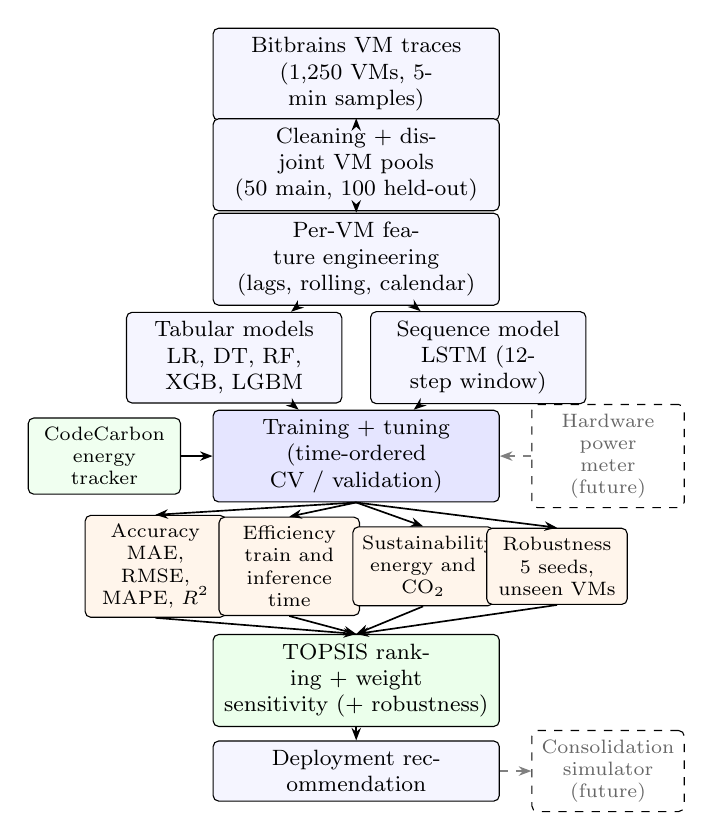
\begin{tikzpicture}[
  box/.style={draw, rounded corners=2pt, align=center, font=\footnotesize, text width=34mm, minimum height=6.5mm, fill=blue!4},
  half/.style={box, text width=25mm},
  quad/.style={draw, rounded corners=2pt, align=center, font=\scriptsize, text width=15.5mm, minimum height=9mm, fill=orange!8},
  side/.style={draw, rounded corners=2pt, align=center, font=\scriptsize, text width=17mm, minimum height=6.5mm},
  fut/.style={side, dashed, text=black!60},
  arr/.style={-{Stealth[length=1.6mm]}, semithick}]
% main flow
\node[box] (raw) at (0, 0) {Bitbrains VM traces\\(1{,}250 VMs, 5-min samples)};
\node[box] (prep) at (0, -1.15) {Cleaning + disjoint VM pools\\(50 main, 100 held-out)};
\node[box] (feat) at (0, -2.35) {Per-VM feature engineering\\(lags, rolling, calendar)};
\node[half] (tab) at (-1.55, -3.6) {Tabular models\\LR, DT, RF, XGB, LGBM};
\node[half] (seq) at (1.55, -3.6) {Sequence model\\LSTM (12-step window)};
\node[box, fill=blue!10] (tune) at (0, -4.85) {Training + tuning\\(time-ordered CV / validation)};
\node[quad] (acc) at (-2.55, -6.25) {Accuracy\\MAE, RMSE,\\MAPE, $R^2$};
\node[quad] (eff) at (-0.85, -6.25) {Efficiency\\train and\\inference time};
\node[quad] (sus) at (0.85, -6.25) {Sustainability\\energy and\\CO$_2$};
\node[quad] (rob) at (2.55, -6.25) {Robustness\\5 seeds,\\unseen VMs};
\node[box, fill=green!8] (topsis) at (0, -7.7) {TOPSIS ranking + weight\\sensitivity (+ robustness)};
\node[box] (rec) at (0, -8.85) {Deployment recommendation};
% side inputs and planned extensions
\node[side, fill=green!6, left=4mm of tune] (cc) {CodeCarbon\\energy tracker};
\node[fut, right=4mm of tune] (meter) {Hardware power\\meter (future)};
\node[fut, right=4mm of rec] (sim) {Consolidation\\simulator (future)};
% arrows
\draw[arr] (raw) -- (prep);
\draw[arr] (prep) -- (feat);
\draw[arr] (feat) -- (tab);
\draw[arr] (feat) -- (seq);
\draw[arr] (tab) -- (tune);
\draw[arr] (seq) -- (tune);
\foreach \n in {acc, eff, sus, rob} { \draw[arr] (tune.south) -- (\n.north); \draw[arr] (\n.south) -- (topsis.north); }
\draw[arr] (topsis) -- (rec);
\draw[arr] (cc) -- (tune);
\draw[arr, dashed, black!50] (meter) -- (tune);
\draw[arr, dashed, black!50] (rec) -- (sim);
\end{tikzpicture}}
\caption{Proposed energy-aware evaluation framework. Dashed boxes are planned extensions that were not implemented.}
\label{fig:pipeline}
\end{figure}

\subsection{Feature Engineering}
Each training example describes one VM at reading $t$ and asks the model to predict its CPU utilization at the next reading, $t+1$, five minutes later. The inputs, listed in Table~\ref{tab:features}, describe the current state of the VM, its recent history (the \emph{lag} features, i.e.\ the values one, two and three readings earlier) and its behaviour over the last half hour (the \emph{rolling} mean and standard deviation over six readings). All features are computed separately for each VM and use only information available at time $t$. Memory is expressed as a percentage of the allocated memory so that VMs of different sizes are comparable. We checked programmatically that no future information leaks into the inputs: the target equals the next reading of the same VM, the lag features equal earlier readings, and no input duplicates the target. The first five and the last reading of each VM, which lack a full history or a next value, are dropped.

\begin{table}[!htb]
\centering
\caption{Model Input Features (Target: CPU Usage at $t+1$)}
\label{tab:features}
\footnotesize
\setlength{\tabcolsep}{3pt}
\begin{tabular}{lp{5.4cm}}
\toprule
Group & Features \\
\midrule
Current & CPU usage (\%), memory usage (\% of provisioned) at $t$ \\
Lags & CPU and memory usage at $t-1$, $t-2$, $t-3$ \\
Rolling & mean and std.\ of CPU usage over $t-5\dots t$ \\
Static$^\dagger$ & provisioned CPU cores \\
I/O$^\dagger$ & disk read/write, network receive/transmit (KB/s) \\
Calendar & hour of day, minute of hour \\
\bottomrule
\end{tabular}
\par\vspace{2pt}
\parbox{\linewidth}{\scriptsize $^\dagger$Removed in the VM-agnostic variant (Section~\ref{sec:m-robust}), leaving 12 of 17 features.}
\end{table}

\subsection{Models}
We compare six models that cover the main families used in the literature, from the simplest to the most complex:
\begin{itemize}
  \item \textbf{Linear Regression (LR)} predicts the target as a weighted sum of the inputs; it is the simplest baseline.
  \item \textbf{Decision Tree (DT)} splits the data by a sequence of if--then rules; it is easy to interpret but can overfit.
  \item \textbf{Random Forest (RF)} \cite{breiman2001rf} averages many decision trees, each trained on a random sample of the data.
  \item \textbf{XGBoost} \cite{chen2016xgboost} and \textbf{LightGBM} \cite{ke2017lightgbm} are \emph{gradient-boosted} tree ensembles: each new tree corrects the errors of the previous ones. Both are widely used for tabular data.
  \item \textbf{LSTM} \cite{hochreiter1997lstm} is a recurrent neural network that reads a sequence of past readings. It is the most common deep-learning model in data-center forecasting \cite{mughees2025stlf,tariq2025nextgen,enyinnah2022lstm,kollu2024comparative}, so including it tests directly whether the higher cost of deep learning buys higher accuracy.
\end{itemize}
The LSTM reads the last 12 readings (one hour) of CPU and memory utilization and has one layer of 64 units. It is trained with the Adam optimizer for at most 15 passes over the data, stopping early once the error on a validation set (the last 10\% of each VM's training period) stops improving. Its input windows may include readings from the training period, so it predicts exactly the same test rows as the other models. The tabular models are implemented with scikit-learn \cite{pedregosa2011sklearn}, XGBoost and LightGBM, and the LSTM with PyTorch \cite{paszke2019pytorch}. As a reference we also report \emph{persistence}, which uses no model at all and simply predicts that the next value equals the current one ($\hat{y}_{t+1}=y_t$); a useful model must beat it. Table~\ref{tab:setup} summarizes the full experimental setup. All experiments ran on the free tier of Google Colab with a CPU-only runtime and no GPU, so all six models were trained on identical hardware and their time and energy can be compared directly.

\begin{table}[!htb]
\centering
\caption{Experimental Setup}
\label{tab:setup}
\footnotesize
\begin{adjustbox}{max width=\columnwidth}
\begin{tabular}{lp{5.2cm}}
\toprule
Setting & Value \\
\midrule
Platform & Google Colab (free), CPU runtime: Intel Xeon 2.20\,GHz, 2 vCPUs, 13.6\,GB RAM \\
Software & Python 3.13, scikit-learn 1.6.1, XGBoost 3.4.1, LightGBM 4.6.0, PyTorch 2.11 (CPU), CodeCarbon 3.3.1 \\
Data & 50 VMs: 321{,}115 train / 80{,}303 test rows; 100 unseen VMs: 815{,}778 rows \\
Target & CPU utilization at $t+1$ (5\,min ahead) \\
Tree tuning & GridSearchCV, time-ordered TimeSeriesSplit (3 folds), RMSE \\
Search spaces & DT: depth $\{5,10,15,\infty\}$ $\times$ min.\ split $\{2,10,50\}$; RF: (50 trees, depth $\{10,20,\infty\}$), (100 trees, depth $\{10,20\}$); XGB/LGBM: trees $\{100,300\}$ $\times$ depth $\{4,6,8\}$ / $\{4,8,\infty\}$ $\times$ lr $\{0.05,0.1\}$; LSTM: units $\{32,64\}$ $\times$ window $\{6,12\}$ \\
Selected & DT depth 5, split 10; RF 100 trees, depth 10; XGB 300 trees, depth 4, lr 0.1; LGBM 300 trees, unlimited depth, lr 0.05; LSTM 32 units, 12 steps \\
LSTM & 1 layer, 64 units, 12-step window, Adam ($10^{-3}$), batch 256, $\leq$15 epochs, patience 3 \\
Seeds & 42 (stability: 42, 7, 123, 2024, 99) \\
Energy & CodeCarbon machine mode, 1\,s sampling, runs repeated to $\geq$30\,s \\
Grid intensity & 0.369\,kg\,CO$_2$/kWh (USA) \\
\bottomrule
\end{tabular}
\end{adjustbox}
\end{table}

\subsection{Hyperparameter Tuning}
Hyperparameters are the settings of a model that are fixed before training, such as the number of trees or their depth. The tree models are tuned with an exhaustive grid search: every combination of settings is tried and scored with three-fold time-series cross-validation. To make each fold a genuine forecast, the training rows are first ordered by time, so that every fold trains on earlier weeks and is scored on the following week; without this ordering the folds would be groups of VMs rather than periods of time. The setting with the lowest average error (RMSE) is then retrained on the full training set. A full grid search with cross-validation is too expensive for the LSTM on free cloud hardware, so it is tuned by trying four configurations and keeping the one with the lowest validation error. The search spaces and the selected settings are listed in Table~\ref{tab:setup}. The Random Forest grid was reduced to five points after a timing study showed that full-depth forests with 100--200 trees take 13--26 minutes per fit.


\subsection{Evaluation Criteria}
\textit{Prediction accuracy} is measured on the test set with four standard measures, where $y_i$ is the actual and $\hat{y}_i$ the predicted CPU utilization. The mean absolute error (MAE) is the average size of an error in CPU percentage points; the root mean squared error (RMSE) gives more weight to large errors; the mean absolute percentage error (MAPE) expresses the error relative to the actual value; and the coefficient of determination ($R^2$) is the share of the variation in CPU load that the model explains (1 is perfect). Lower is better for the first three and higher is better for $R^2$:
\begin{equation}
\mathrm{MAE}=\tfrac{1}{n}\textstyle\sum_{i}|y_i-\hat{y}_i|,\quad
\mathrm{RMSE}=\sqrt{\tfrac{1}{n}\textstyle\sum_{i}(y_i-\hat{y}_i)^2},
\end{equation}
\begin{equation}
\mathrm{MAPE}=\tfrac{100}{|S|}\textstyle\sum_{i\in S}\left|\tfrac{y_i-\hat{y}_i}{y_i}\right|,\quad
R^2=1-\tfrac{\sum_i (y_i-\hat{y}_i)^2}{\sum_i (y_i-\bar{y})^2},
\end{equation}
where $S$ contains the test points with $y_i\geq1\%$; MAPE cannot be computed when the actual value is close to zero, which is common for idle VMs (62.6\% of test points are included). \textit{Computational efficiency} is measured as the training time of one run and the prediction (inference) time per 1{,}000 predictions. \textit{Environmental sustainability} is measured as the energy (kWh) and CO$_2$ emissions (kg) of one training run.

\subsection{Energy and Carbon Measurement}
Energy is measured with CodeCarbon \cite{courty2024codecarbon}, an open-source tool that measures or, where hardware sensors are unavailable, estimates the power drawn by the processor and memory every second while the code runs (Section~\ref{sec:limitations}). Very short runs are hard to measure precisely, so models that train in under 30\,s are trained repeatedly until about 30\,s have passed, and the total is divided by the number of repetitions. CO$_2$ emissions are computed as the measured energy multiplied by the carbon intensity of the local electricity grid (kg of CO$_2$ per kWh), taken from CodeCarbon's data tables for the detected location. We do not use CodeCarbon's own emission total because, for short runs, its ratio to the measured energy varied between runs at the same location; for the same reason, the location is fixed at the first measurement of each session. All models compared within one ranking are measured in the same session, on the same machine.

\subsection{Stability Testing}
Several models involve randomness during training, for example the random samples drawn by Random Forest or the random starting weights of the LSTM. To check that differences between models are genuine and not luck, every tuned model is retrained with five different random seeds (42, 7, 123, 2024 and 99), and we report the mean and standard deviation of MAE, RMSE and $R^2$.

\subsection{TOPSIS Ranking and Sensitivity Analysis}
\label{sec:m-topsis}
TOPSIS \cite{hwang1981topsis} turns several criteria into one score. The idea is simple: imagine an \emph{ideal} model that has the best value of every criterion and an \emph{anti-ideal} model that has the worst value of every criterion; a model is ranked higher the closer it is to the ideal and the farther it is from the anti-ideal. Formally, let $x_{ij}$ be the value of criterion $j$ for model $i$. TOPSIS first rescales each criterion so that criteria measured in different units (seconds, grams, percentage points) become comparable, and multiplies it by its weight $w_j$:
\begin{equation}
r_{ij}=\frac{x_{ij}}{\sqrt{\sum_{k}x_{kj}^2}},\qquad v_{ij}=w_j\,r_{ij},
\end{equation}
It then takes the ideal value $v_j^+$ of each criterion (the maximum for criteria where higher is better, the minimum for criteria where lower is better) and the anti-ideal value $v_j^-$, measures each model's distances $D_i^+$ and $D_i^-$ to the ideal and the anti-ideal model, and ranks the models by the closeness coefficient $C_i$, which lies between 0 and 1 (higher is better):
\begin{equation}
C_i=\frac{D_i^-}{D_i^++D_i^-},\quad D_i^{\pm}=\sqrt{\textstyle\sum_j\left(v_{ij}-v_j^{\pm}\right)^2}.
\end{equation}
We use six criteria: MAE, RMSE, MAPE, training time and CO$_2$ (lower is better) and $R^2$ (higher is better). The primary weights are MAE 0.15, RMSE 0.15, MAPE 0.15, $R^2$ 0.20, training time 0.15 and CO$_2$ 0.20. Accuracy keeps 0.65 of the total weight because a poor forecast leads to over- or under-provisioning, whose energy and service costs far exceed the cost of training the model. $R^2$ receives slightly more weight than each error measure because it summarizes overall fit independently of scale, and CO$_2$ receives the highest single cost weight because it is the focus of this work. Since any choice of weights is partly subjective, we repeat the ranking under four further scenarios (Balanced: every criterion $1/6$; Accuracy-Priority: accuracy 0.80 in total; Energy-Priority: CO$_2$ 0.45; Speed-Priority: training time 0.45) and in a continuous sweep that moves the total weight on cost from 0 to 1.

\subsection{Generalization and Robustness Extensions}
\label{sec:m-robust}
\textit{Unseen VMs.} To test whether the models work on machines they have never seen, the trained models are applied, unchanged, to the 100 held-out VMs (815{,}778 predictions).

\textit{VM-agnostic features.} Some inputs describe a particular machine rather than its load, namely the number of cores and the disk and network activity. To test whether these inputs limit generalization, we retrain each tabular model on a \emph{VM-agnostic} feature set without them (Table~\ref{tab:features}).

\textit{Robustness-aware ranking.} We add unseen-VM MAE to TOPSIS as a seventh criterion (weights: MAE 0.10, RMSE 0.10, MAPE 0.10, $R^2$ 0.15, unseen-VM MAE 0.20, training time 0.15, CO$_2$ 0.20).

\textit{Significance tests.} To check whether differences between two models are statistically meaningful, we compare their per-VM errors with the paired Wilcoxon signed-rank test \cite{wilcoxon1945} and the paired $t$-test, and their individual forecast errors with the Diebold--Mariano test \cite{diebold1995dm}, the standard test for comparing two forecasting models (with a Newey--West correction for correlated errors, lag 12).

\textit{Fleet projection.} Finally, the measured training and prediction energy is scaled up to a hypothetical fleet of 10{,}000 VMs.

% =====================================================================
\section{Experimental Results and Discussion}
\label{sec:results}

\subsection{Predictive Accuracy}
\textit{The three tree ensembles are the most accurate models, and the LSTM is not.} Table~\ref{tab:results} reports all tuned models on the test set. LightGBM is the most accurate model on every measure: its forecasts are off by 0.664 percentage points of CPU on average (MAE), and it explains 94.1\% of the variation in CPU load ($R^2=0.941$). XGBoost and Random Forest follow closely. The LSTM (MAE 0.924) is less accurate than all three ensembles. Only the ensembles beat the no-model persistence reference on both MAE and RMSE; persistence is a strong reference here because many VMs stay idle for long periods. Fig.~\ref{fig:actualpred} shows that all models follow the bursty load of a representative VM, with the largest errors at sudden jumps.

\begin{table*}[!b]
\centering
\caption{Accuracy, Cost, Energy and TOPSIS Ranking of the Tuned Models (Test Set)}
\label{tab:results}
\footnotesize
\setlength{\tabcolsep}{4pt}
\begin{adjustbox}{max width=\textwidth}
\begin{tabular}{lrrrrrrrrrr}
\toprule
Model & MAE & RMSE & MAPE\% & R$^2$ & Train s & Inf.\,ms/1k & Wh & g\,CO$_2$ & $C_i$ & Rank \\
\midrule
LR & 0.903 & 4.590 & 18.24 & 0.9062 & \textbf{0.253} & 0.286 & \textbf{0.0011} & \textbf{0.00041} & 0.869 & 3 \\
DT & 1.050 & 4.356 & 28.07 & 0.9156 & 2.04 & \textbf{0.111} & 0.008 & 0.003 & 0.762 & 4 \\
RF & 0.697 & 3.749 & 14.04 & 0.9374 & 195 & 3.46 & 0.95 & 0.35 & 0.220 & 6 \\
XGB & 0.697 & 3.715 & 13.43 & 0.9386 & 5.92 & 4 & 0.022 & 0.0083 & \textbf{0.968} & 1 \\
LGBM & \textbf{0.664} & \textbf{3.651} & \textbf{12.42} & \textbf{0.9407} & 7.82 & 6.94 & 0.034 & 0.013 & 0.965 & 2 \\
LSTM & 0.924 & 4.494 & 19.74 & 0.9101 & 159 & 13.6 & 0.76 & 0.28 & 0.229 & 5 \\
\textit{Persist.} & 0.733 & 4.657 & 13.92 & 0.9035 & 0 & -- & 0 & 0 & -- & -- \\
\bottomrule
\end{tabular}
\end{adjustbox}
\par\vspace{3pt}
{\scriptsize Best value per column in bold. Energy and CO$_2$ are per training run (CodeCarbon; USA/Iowa grid, 0.369 kg/kWh). Inference time per 1{,}000 predictions. Persist.: persistence reference ($\hat{y}_{t+1}=y_t$), not ranked.\par}
\end{table*}


\begin{figure}[!htb]
\centering
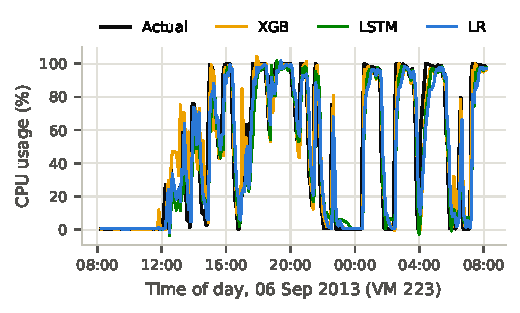
\includegraphics[width=\columnwidth]{fig_actual_vs_predicted_col.pdf}
\caption{Actual and predicted CPU utilization for VM 223 over the first 24 hours of the test period (TOPSIS winner XGBoost, LSTM and Linear Regression).}
\label{fig:actualpred}
\end{figure}

\subsection{Computational Cost, Energy and Emissions}
\textit{The most expensive models are not the most accurate.} The cost of training differs by a factor of more than 800 between the cheapest and the most expensive model (Table~\ref{tab:results}). One training run of the tuned LightGBM takes 7.8\,s and 0.034\,Wh, whereas Random Forest and the LSTM need 195\,s and 159\,s and consume 28 and 22 times more energy. With default settings the gap is even larger: the default Random Forest trains for 612\,s and the LSTM for 218\,s, about 260 and 90 times the energy of LightGBM. Fig.~\ref{fig:tradeoff} plots accuracy against CO$_2$; a plot against training time looks the same, because on this hardware the two are almost perfectly correlated. Linear Regression, XGBoost and LightGBM lie on the \emph{Pareto front}, meaning that no other model is both more accurate and cheaper. Random Forest and the LSTM are \emph{dominated}: another model beats them on accuracy and on cost at the same time. Average power was similar for all models (13.7--17.5\,W), so the differences in energy come mainly from differences in run time.

\begin{figure}[!htb]
\centering
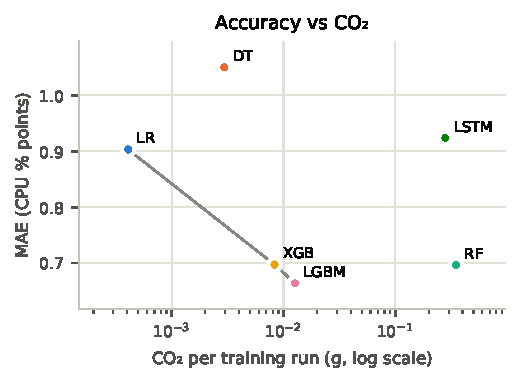
\includegraphics[width=\columnwidth]{fig_tradeoff_accuracy_vs_energy.pdf}
\caption{Trade-off between test MAE and CO$_2$ per training run (log scale). The grey line joins the Pareto-optimal models; the chart against training time is nearly identical.}
\label{fig:tradeoff}
\end{figure}

\subsection{Cost and Benefit of Hyperparameter Tuning}
\textit{Tuning cost more energy than it returned in accuracy.} Table~\ref{tab:tuning} compares the default and tuned versions of each model. Tuning took 53.4 minutes in total and an estimated 15.2\,Wh (5.6\,g CO$_2$), more than training all six final models once, yet it lowered MAE by only 1.5\% for LightGBM and 0.5\% for XGBoost. Random Forest used 69\% of the tuning time and became slightly less accurate on the test set, and the LSTM's four configurations differed by less than 1\% in validation error. Because the search minimizes RMSE, the Decision Tree's RMSE improved by 17\% while its MAE became worse. One useful side effect is that the tuned Random Forest (with trees limited to depth 10) trains 2.6 times faster than the default one.

\begin{table}[!htb]
\centering
\caption{Effect and Cost of Hyperparameter Tuning (Test Set)}
\label{tab:tuning}
\footnotesize
\setlength{\tabcolsep}{4pt}
\begin{adjustbox}{max width=\columnwidth}
\begin{tabular}{lrrrrrrr}
\toprule
Model & MAE$_{def}$ & MAE$_{tun}$ & $\Delta$\% & RMSE$_{def}$ & RMSE$_{tun}$ & Min & Wh \\
\midrule
LR & 0.903 & 0.903 & +0.0 & 4.590 & 4.590 & 0.0 & -- \\
DT & 0.847 & 1.050 & +24.0 & 5.247 & 4.356 & 1.9 & 0.46 \\
RF & 0.690 & 0.697 & +0.9 & 3.685 & 3.749 & 37.0 & 11 \\
XGB & 0.701 & 0.697 & -0.5 & 3.738 & 3.715 & 2.8 & 0.64 \\
LGBM & 0.674 & 0.664 & -1.5 & 3.712 & 3.651 & 2.4 & 0.63 \\
LSTM & 0.877 & 0.924 & +5.3 & 4.534 & 4.494 & 9.2 & 2.7 \\
\bottomrule
\end{tabular}
\end{adjustbox}
\par\vspace{3pt}
{\scriptsize Wh: estimated tuning energy = tuning time $\times$ measured mean power of that model.\par}
\end{table}


\subsection{Stability Across Random Seeds}
\textit{The tree models give the same answer every time; the LSTM does not.} Across the five seeds, XGBoost, Linear Regression and the Decision Tree give identical results, and Random Forest ($0.697\pm0.003$ MAE) and LightGBM ($0.661\pm0.003$) vary only in the third decimal. LightGBM is the most accurate model for every seed, and its lead over the runner-up (0.036 MAE) is more than ten times the seed-to-seed variation, so it is not due to chance. The LSTM is the least stable model ($0.942\pm0.061$ MAE; its variation relative to its mean is about 15 times that of the ensembles), so retraining it can produce a noticeably different model.


\subsection{TOPSIS Ranking and Weight Sensitivity}
\textit{The two boosted-tree models are recommended under every realistic weighting.} With the primary weights, TOPSIS ranks XGBoost first ($C=0.968$) and LightGBM a very close second ($0.965$), followed by Linear Regression, the Decision Tree, the LSTM and Random Forest (Fig.~\ref{fig:topsis}a, Table~\ref{tab:results}). LightGBM is more accurate, but the tuned XGBoost trained faster on this hardware, which tips the cost criteria in its favour; in practice the two are tied. Fig.~\ref{fig:topsis}b shows that XGBoost ranks first in four of the five weighting scenarios and LightGBM under Accuracy-Priority, while Random Forest and the LSTM take the last two places in every scenario. In the continuous sweep, LightGBM wins when cost carries less than 35\% of the weight, XGBoost between 35\% and 75\%, and Linear Regression only above 80\%. On this hardware training time and CO$_2$ are almost perfectly correlated (correlation 0.9999), so we also merged them into a single cost criterion; every rank stayed the same.

\begin{figure}[!htb]
\centering
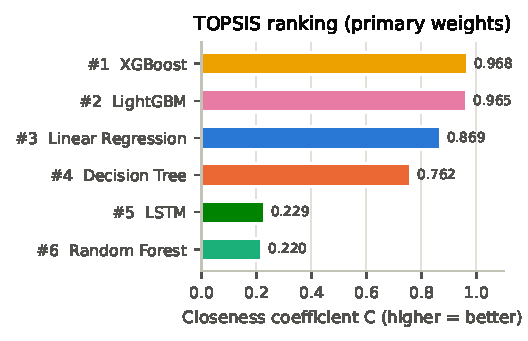
\includegraphics[width=0.82\columnwidth]{fig_topsis_ranking.pdf}\\[2pt]
{\footnotesize (a)}\\[4pt]
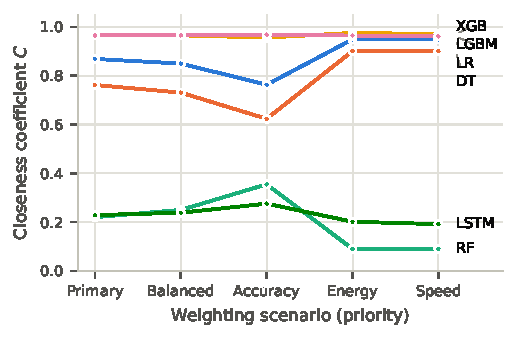
\includegraphics[width=\columnwidth]{fig_topsis_sensitivity_col.pdf}\\[2pt]
{\footnotesize (b)}
\caption{(a) TOPSIS closeness with the primary weights. (b) Closeness under the five weighting scenarios.}
\label{fig:topsis}
\end{figure}

\subsection{Generalization to Unseen VMs}
\textit{On machines the models have never seen, the accuracy ranking reverses.} Table~\ref{tab:generalization} reports the tuned models on the 100 VMs that were never used for training or tuning. Here the LSTM (MAE 0.696) and Linear Regression (0.707) are the most accurate, whereas LightGBM (1.083) and Random Forest (1.095) fall behind. The rank correlation between the test-set and unseen-VM rankings is $-0.09$ ($-0.54$ for the default models), i.e.\ the ranking on known VMs says nothing about the ranking on new ones. The ensembles are still the best on a typical VM (they have the lowest median error per VM) but fail badly on a few VMs. The clearest case is VM~387, which reads heavily from disk (35{,}000\,KB/s on average) while using only about 9\% CPU. In the training VMs heavy disk activity went together with high CPU, so the tree models predict about 60\% CPU for this VM (LightGBM MAE 28.7 on this VM, against 1.06 for the LSTM). No model beats persistence on unseen-VM MAE, although the LSTM does on RMSE.

\begin{table}[!htb]
\centering
\caption{Generalization of the Tuned Models to 100 Unseen VMs}
\label{tab:generalization}
\footnotesize
\setlength{\tabcolsep}{4pt}
\begin{adjustbox}{max width=\columnwidth}
\begin{tabular}{lrrrrrrr}
\toprule
Model & MAE$_{test}$ & MAE$_{unseen}$ & $\Delta$\% & RMSE & R$^2$ & Med. VM & Worst VM \\
\midrule
LR & 0.903 & 0.707 & -21.7 & 3.350 & 0.9612 & 0.258 & 5.3 \\
DT & 1.050 & 1.581 & +50.6 & 5.805 & 0.8836 & 0.561 & 36.6 \\
RF & 0.697 & 1.095 & +57.2 & 4.602 & 0.9269 & 0.182 & 29.7 \\
XGB & 0.697 & 0.919 & +31.8 & 3.385 & 0.9604 & 0.192 & 10.5 \\
LGBM & 0.664 & 1.083 & +63.0 & 4.476 & 0.9308 & 0.159 & 28.7 \\
LSTM & 0.924 & 0.696 & -24.7 & 3.235 & 0.9639 & 0.255 & 5.0 \\
\textit{Persist.} & 0.733 & 0.506 & -- & 3.315 & 0.9620 & -- & -- \\
\bottomrule
\end{tabular}
\end{adjustbox}
\par\vspace{3pt}
{\scriptsize Med./Worst VM: median and maximum per-VM MAE over the 100 unseen VMs.\par}
\end{table}


\subsection{VM-Agnostic Features and Robustness-Aware Ranking}
\textit{Removing VM-specific features largely fixes the problem.} Fig.~\ref{fig:ablation} compares each model trained with all 17 features (solid bars) and with the 12 VM-agnostic features (hatched bars). Without the core count and the four disk and network features, LightGBM's error on unseen VMs falls by 30\% (MAE 0.972 to 0.681), and its error on the worst VM falls from 34.7 to 4.6; on VM~387 it drops from 34.7 to 1.5. Random Forest improves by 21\% (worst VM 30.4 to 8.7), the Decision Tree by 33\%, XGBoost by 12\% and Linear Regression by 9\%; the VM-agnostic Linear Regression (0.645) and LightGBM (0.681) are then the most accurate models on unseen VMs. The price is a 6--10\% higher error for the ensembles on the known VMs. In other words, the disk and network features help on the training machines but act as a ``fingerprint'' of individual VMs that does not carry over to new ones. (The full-feature LightGBM in Fig.~\ref{fig:ablation} was retrained with a different row order; its unseen-VM MAE of 0.972 instead of 1.083 shows how unstable it is on unusual VMs.)

\begin{figure*}[!t]
\centering
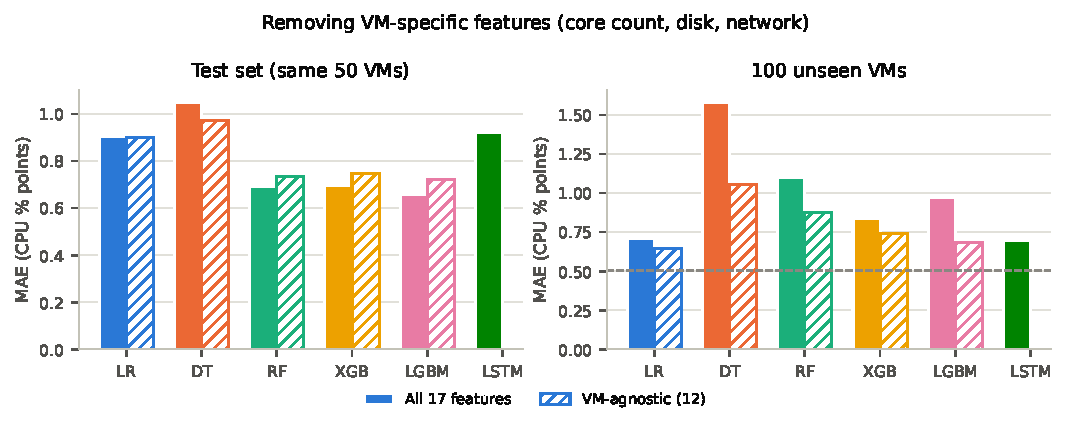
\includegraphics[width=0.92\textwidth]{fig_ablation_generalization.pdf}
\caption{MAE of full-feature (solid) and VM-agnostic (hatched) models on the test set and on 100 unseen VMs. The dashed line marks persistence on the unseen VMs.}
\label{fig:ablation}
\end{figure*}


\textit{Including robustness changes the recommendation.} Table~\ref{tab:robust} ranks all 11 model variants (six full-feature models and five VM-agnostic ones). Standard TOPSIS selects the full-feature XGBoost, whereas robustness-aware TOPSIS, which also rewards accuracy on unseen VMs, selects the VM-agnostic LightGBM ($C=0.967$), followed by the VM-agnostic XGBoost. The VM-agnostic LightGBM takes the lead as soon as unseen-VM MAE receives a weight of 0.10, and the VM-agnostic Linear Regression only above 0.60. The LSTM and Random Forest occupy the bottom three places in both rankings.

\begin{table}[!htb]
\centering
\caption{Standard vs. Robustness-Aware TOPSIS (11 Variants)}
\label{tab:robust}
\footnotesize
\setlength{\tabcolsep}{4pt}
\begin{adjustbox}{max width=\columnwidth}
\begin{tabular}{lrrrr}
\toprule
Variant & $C_i$ std. & Rank & $C_i$ robust & Rank \\
\midrule
LGBM-A & 0.960 & 3 & 0.967 & 1 \\
XGB-A & 0.951 & 4 & 0.953 & 2 \\
XGB & 0.969 & 1 & 0.930 & 3 \\
LR-A & 0.885 & 5 & 0.924 & 4 \\
LR & 0.884 & 6 & 0.920 & 5 \\
LGBM & 0.963 & 2 & 0.886 & 6 \\
DT-A & 0.830 & 7 & 0.831 & 7 \\
DT & 0.787 & 8 & 0.714 & 8 \\
LSTM & 0.325 & 9 & 0.401 & 9 \\
RF-A & 0.262 & 10 & 0.302 & 10 \\
RF & 0.199 & 11 & 0.195 & 11 \\
\bottomrule
\end{tabular}
\end{adjustbox}
\par\vspace{3pt}
{\scriptsize Robust weights: MAE .10, RMSE .10, MAPE .10, R$^2$ .15, unseen MAE .20, training time .15, CO$_2$ .20.\par}
\end{table}


\subsection{Statistical Significance}
\textit{LightGBM is better on a typical machine; XGBoost is safer in the worst case.} On the test set LightGBM has a lower MAE than XGBoost (paired $t$-test over VMs, $p=0.005$; Diebold--Mariano, $p<0.001$), although it is better on only 27 of the 50 VMs (Wilcoxon, $p=0.08$). On the unseen VMs LightGBM is better on 71 of 100 VMs (Wilcoxon, $p<0.001$), yet XGBoost has the lower average error because LightGBM fails badly on a few VMs (paired $t$-test, $p=0.71$). LightGBM also outperforms the LSTM on 46 of 50 test VMs ($p<0.001$), whereas the LSTM is more accurate on the unseen VMs (Diebold--Mariano, $p<0.001$). The Diebold--Mariano test treats tens of thousands of correlated forecast errors as evidence and therefore tends to report very small $p$-values; we regard the VM-level tests as the more conservative evidence.

\subsection{Fleet-Scale Projection}
\textit{Retraining, not prediction, dominates the energy of a deployed forecaster.} To put the measurements in context, we scale them to a hypothetical fleet of 10{,}000 VMs served by 200 models (one per group of 50 VMs) that are retrained daily and produce a forecast for every VM every 5 minutes ($1.05\times10^9$ predictions per year). Annual CO$_2$ ranges from 0.018\,kg for the VM-agnostic Linear Regression and 0.64\,kg for the VM-agnostic LightGBM to 17\,kg for the LSTM and 25\,kg for Random Forest, a spread of more than 1{,}000 times. Training accounts for more than 97\% of the total for every model, so retraining frequency is the dominant lever. In absolute terms these amounts are small compared with the energy of the servers being forecast.


\subsection{Discussion: Why Accuracy-Only Selection Is Misleading}
\label{sec:discussion}
Accuracy-only selection is misleading in two ways. First, it hides a large cost gap: models within 0.04 MAE of each other differ by 20--30 times in training energy, and the most expensive models are not the most accurate. Second, it can select models that do not transfer: the most accurate models on known VMs were among the least accurate on new VMs. A multi-criteria procedure that includes cost and robustness avoids both errors.

\subsection{Discussion: Does Deep Learning Justify Its Cost?}
In our setting it does not. The LSTM needed 22 times the training energy of the tuned LightGBM, was less accurate on known VMs, was the least stable model across seeds and was the slowest at inference, and it ranked fifth or sixth in every TOPSIS scenario. Its good unseen-VM accuracy stems from using only utilization history, an advantage that the VM-agnostic LightGBM matches at a fraction of the cost. This agrees with evidence that tree ensembles and simple linear models are hard to beat on tabular and short-horizon forecasting tasks \cite{grinsztajn2022tree,zeng2023transformers} and with Green AI findings in other domains \cite{vente2024clicks,barros2025small}.

\subsection{Implications for Cloud Providers}
Our results lead to five practical recommendations:
\begin{enumerate}
  \item \textbf{Use gradient-boosted trees as the default} for VM load forecasting: they are accurate, stable and cheap to retrain.
  \item \textbf{Treat features that identify a VM with care}, such as its resource configuration or disk and network signature, and always validate a model on held-out VMs before deploying it across a fleet.
  \item \textbf{Keep hyperparameter searches small}: on this task the search used more energy than training all final models, for at most a 1.5\% gain.
  \item \textbf{Prefer fast-training models}, because retraining dominates the lifetime energy of a forecaster and its cost grows with the retraining frequency.
  \item \textbf{Always report a persistence baseline}: on mostly idle workloads it is hard to beat, and a model that does not beat it adds cost without benefit.
\end{enumerate}

Finally, the absolute emissions of forecasting models are small next to those of the servers they manage. The value of energy-aware selection therefore lies less in the emissions of a single deployment than in avoiding waste that grows with scale and retraining frequency: in our projection the VM-agnostic LightGBM is more accurate on unseen VMs than Random Forest and the LSTM while emitting 26--39 times less CO$_2$.

% =====================================================================
\section{Limitations and Future Work}
\label{sec:limitations}

\subsection{Limitations}
\textit{Energy measurement.} Cloud VMs do not expose hardware power counters, so CodeCarbon estimated CPU power from the processor's rated power and RAM power from its size. Energy is therefore close to proportional to run time, and absolute values may deviate from metered consumption by up to 40\% \cite{fischer2025groundtruth}; relative comparisons on identical hardware are more reliable than absolute figures. CO$_2$ uses a country-level grid intensity for the detected location.

\textit{Data.} We use one dataset from a single provider, recorded in 2013 and covering one month, with mostly enterprise and financial workloads. Modern AI and GPU workloads and seasonal effects such as quarter-end peaks are not represented, and many VMs are idle, which favors persistence.

\textit{Scope.} The main experiment uses 50 VMs (321{,}115 training rows) and a single 5-minute forecast horizon. Hyperparameter grids were deliberately small to fit free cloud hardware, and the LSTM was tuned over only four configurations, so larger searches might shift individual results. We used one global model per VM group rather than per-VM models, and hardware differences between sessions mean that energy values are comparable only within a session.

\textit{Decision model.} TOPSIS results depend on the chosen weights and criteria; we mitigate this with scenario and sweep analyses, but other MCDM methods may rank close alternatives differently. The fleet projection rests on stated assumptions and excludes data handling and facility overhead (PUE).

\subsection{Future Work}
\begin{enumerate}
  \item validating it on further and more recent traces (e.g., Alibaba and Google cluster data) and on GPU-based AI workloads;
  \item measuring energy with hardware power meters or RAPL counters instead of estimates;
  \item studying multiple forecast horizons, per-VM models and retraining schedules;
  \item extending the comparison to further deep architectures, such as GRUs and lightweight Transformers, and to compression of the selected models;
  \item comparing TOPSIS with other MCDM methods and data-driven weighting schemes;
  \item integrating the selected forecaster into a VM-consolidation simulator to quantify end-to-end data-center energy savings.
\end{enumerate}

% =====================================================================
\section{Conclusion}
\label{sec:conclusion}

We presented an energy-aware evaluation framework that selects workload-forecasting models for cloud data centers on accuracy, computational cost, energy and CO$_2$, stability and generalization, combined through TOPSIS. On real Bitbrains traces, gradient-boosted trees offered the best balance: LightGBM was the most accurate model, and XGBoost ranked first overall with the primary weights. Random Forest and an LSTM consumed 22--28 times more training energy without accuracy gains and ranked last under every weighting, and hyperparameter tuning cost more energy than it returned in accuracy. Testing on unseen VMs revealed that VM-specific I/O features cause tree ensembles to fail on atypical machines; VM-agnostic features reduced LightGBM's unseen-VM error by 30\%, and a robustness-aware TOPSIS ranking recommends this model.

Evaluating forecasting models on cost and robustness, not only on accuracy, leads to cheaper and more reliable deployment choices.

% =====================================================================
\section*{Acknowledgment}
The GWA-T-12 Bitbrains trace was graciously provided by Bitbrains IT Services Inc.\ \cite{shen2015bitbrains} and is distributed through the Grid Workloads Archive \cite{iosup2008gwa} maintained by TU Delft. All code, notebooks, logs and result tables are available from the authors.

\bibliographystyle{IEEEtran}
\bibliography{references}

\end{document}
